%&latex
%
\documentclass[../template.tex]{subfiles}

\begin{document}

\section{Numerical methods}

...Recover first part...

So the \textbf{strategy} is to choose a subset of states $M$:
\begin{align*}
    \langle Q \rangle \approx \frac{\displaystyle \sum_{i=1}^M Q_{Mi} e^{- \beta E_{M_i}}}{\sum_{t=1}^M e^{-\beta E_{M_t}}} 
\end{align*} 
This can be done because typically the system explores a very small region amongst all the possible states.
For example, when launching two dice, their sum will usually be around $7$, because there are many combinations allowing it.

\medskip

So we want to choose a subset that is \textit{relevant} for the system at hand. This is done with \textbf{importance sampling}. The idea is just to sample with a Boltzmann probability:
\begin{align*}
    \langle Q \rangle = \frac{1}{M} \sum_{i=1}^M Q_{M_i} \qquad P_{M_i} = \frac{e^{-\beta E_{M_i}}}{Z}  
\end{align*}   

First, let's review briefly Markov Processes. A Markov Process is a mechanism which, when given a system state $\mu$, is able to generate a new state $\nu$. In other words, all relevant information necessary for the system's evolution is contained in the starting state - no additional quantities are required. 

The probability of going from $\mu$ and $\nu$ is the \textbf{transition probability} between the two states, and it is denoted as $\mathbb{P}(\mu \to \nu)$.

It satisfies the following properties:
\begin{enumerate}
    \item $\mathbb{P}(\mu \to \nu)$ is independent of time
    \item $\mathbb{P}(\mu \to \nu)$ does not depend on the \q{past history} of the system states. In other words, the process is \textit{memoryless}.
    \item \textbf{Normalization} 
    \begin{align*}
        \sum_{\nu} \mathbb{P}(\mu \to \nu) = 1        
    \end{align*}
    Note that, in general, $\mathbb{P}(\mu \to \nu) \neq 0$.
\end{enumerate}

We will now show that if we generate states through a Markov Process satisfying \textbf{ergodicity} and \textbf{detailed balance}, then we are generating samples according to a Boltzmann distribution. 

\begin{itemize}
    \item \textbf{Ergodicity}: it is possible to reach any state of the system from any other state. 
    \item \textbf{Detailed balance}: a necessary condition to have equilibrium is that the probability of \textit{exiting} a state $\mu$ must be the same of that of \textit{entering} it. %Add drawing
    More precisely:
    \begin{align}\label{eqn:db}
        \sum_\nu \mathbb{P}(\mu) \mathbb{P}(\mu \to \nu)= \sum_\nu P_\nu \mathbb{P}(\nu \to \mu)
    \end{align}  
    Intuitively, this means that there is no net \q{probability flux} between nodes at equilibrium. Equivalently:
    \begin{align*}
        P_{\mu} = \sum_{\nu} P_{\nu} \mathbb{P}(\nu \to \mu)
    \end{align*} 
    which follows directly from (\ref{eqn:db}):
    \begin{align*}
        \sum_{\nu} \hlc{Yellow}{\mathbb{P}(\mu)} \mathbb{P}(\mu \to \nu) = \sum_\nu \hlc{Yellow}{ \sum_\nu \mathbb{P}(\nu) \mathbb{P}(\nu \to \mu)} \mathbb{P}(\mu \to \nu)
    \end{align*}
    Because of ergodicity:
    \begin{align*}
        \sum_\nu \mathbb{P}(\mu \to \nu) = 1 = \sum_\nu \mathbb{P}(\nu) \mathbb{P}(\nu \to \mu)
    \end{align*} %Fix
    And so:
    \begin{align*}
        \mathbb{P}(\mu) = \sum_{\nu} \mathbb{P}(\nu) \mathbb{P}(\nu \to \mu)
    \end{align*}
    Now denote the transition probabilities as:
    \begin{align*}
        A_{\mu \nu} \equiv \mathbb{P}(\nu \to \mu)
    \end{align*}
    Consider the matrix $A$ of entries $A_{\mu \nu}$.
    In vector notation, the system's evolution is described by:
    \begin{align*}
        \bm{P}_{t+1} = A \bm{P}(t)
    \end{align*}
    At stationarity, i.e. for $t \to \infty$, we have:
    \begin{align*}
        \bm{P}_{\infty} = A \bm{P}_\infty
    \end{align*}
    The solution for $\bm{P}_\infty$ is called a \textbf{simple equilibrium}. 
    
    \medskip

    Note, however, that this is not the unique solution. Another possible solution is given by:
    \begin{align*}
        \bm{P}_\infty = A^n \bm{P}_\infty
    \end{align*}
    where the system \textit{cycles} between $n$ states. %Drawing
    
    For example, for $n=3$:
    \begin{align*}
        \left(\begin{array}{c}
        1 \\ 
        0 \\ 
        0
        \end{array}\right) \to \left(\begin{array}{c}
        0 \\ 
        1 \\ 
        0
        \end{array}\right) \to \left(\begin{array}{c}
        0 \\ 
        0 \\ 
        1
        \end{array}\right) \to \left(\begin{array}{c}
        1 \\ 
        0 \\ 
        0
        \end{array}\right)
    \end{align*}
    This is a forme of \textbf{dynamic equilibrium}. The stationarity condition holds:
    \begin{align*}
        \sum_\nu P_\mu P(\mu \to \nu) = \sum_\nu P_\nu \mathbb{P}(\nu \to \mu)
    \end{align*} 
    But in the dynamic equilibrium case we have a flux of probability between different states, and so detailed balance does not hold.

    \medskip

    To eliminate the cycles we impose the following (stronger) condition:
    \begin{align}\label{eqn:detailed-balance}
        \mathbb{P}_{\mu} \mathbb{P}(\mu \to \nu) = \mathbb{P}_{\nu} \mathbb{P}(\nu \to \mu)
    \end{align}
\end{itemize}

The Boltzmann distribution naturally obeys ergodicity:
\begin{align*}
    P_{\mu} \sim e^{-\beta E_{\mu}} > 0
\end{align*}
Note that this does not imply that all transition probabilities must be non-zero, but simply that there must be at least one \textit{path} of non-zero probability connecting every pair of states.

\medskip

Moreover, it obeys detailed balance:
\begin{align*}
    \mathbb{P}_\mu \mathbb{P}(\mu \to \nu) = \mathbb{P}_\nu \mathbb{P}(\nu \to \mu) \Rightarrow \frac{\mathbb{P}(\mu \to \nu)}{\mathbb{P}(\nu \to \mu)}  = \frac{P_\nu}{P_\mu} = \frac{e^{- \beta \mathcal{E}_\nu}}{\cancel{Z}} \frac{\cancel{Z}}{e^{-\beta \mathcal{E}_\nu}}   
\end{align*}
and so:
\begin{align}\label{eqn:boltz-db}
    \frac{\mathbb{P}(\mu \to \nu)}{\mathbb{P}(\nu \to \mu)} = e^{- \beta (\mathcal{E}_\nu - \mathcal{E}_\mu)}  
\end{align}

So, if we use a Markov Process obeying (\ref{eqn:boltz-db}) and it is \textbf{ergodic}, then $P_\mu$ is a Boltzmann distribution. So we can use it to simulate the system.  

\begin{comment}
\begin{figure}[hbp]
    \centering
    %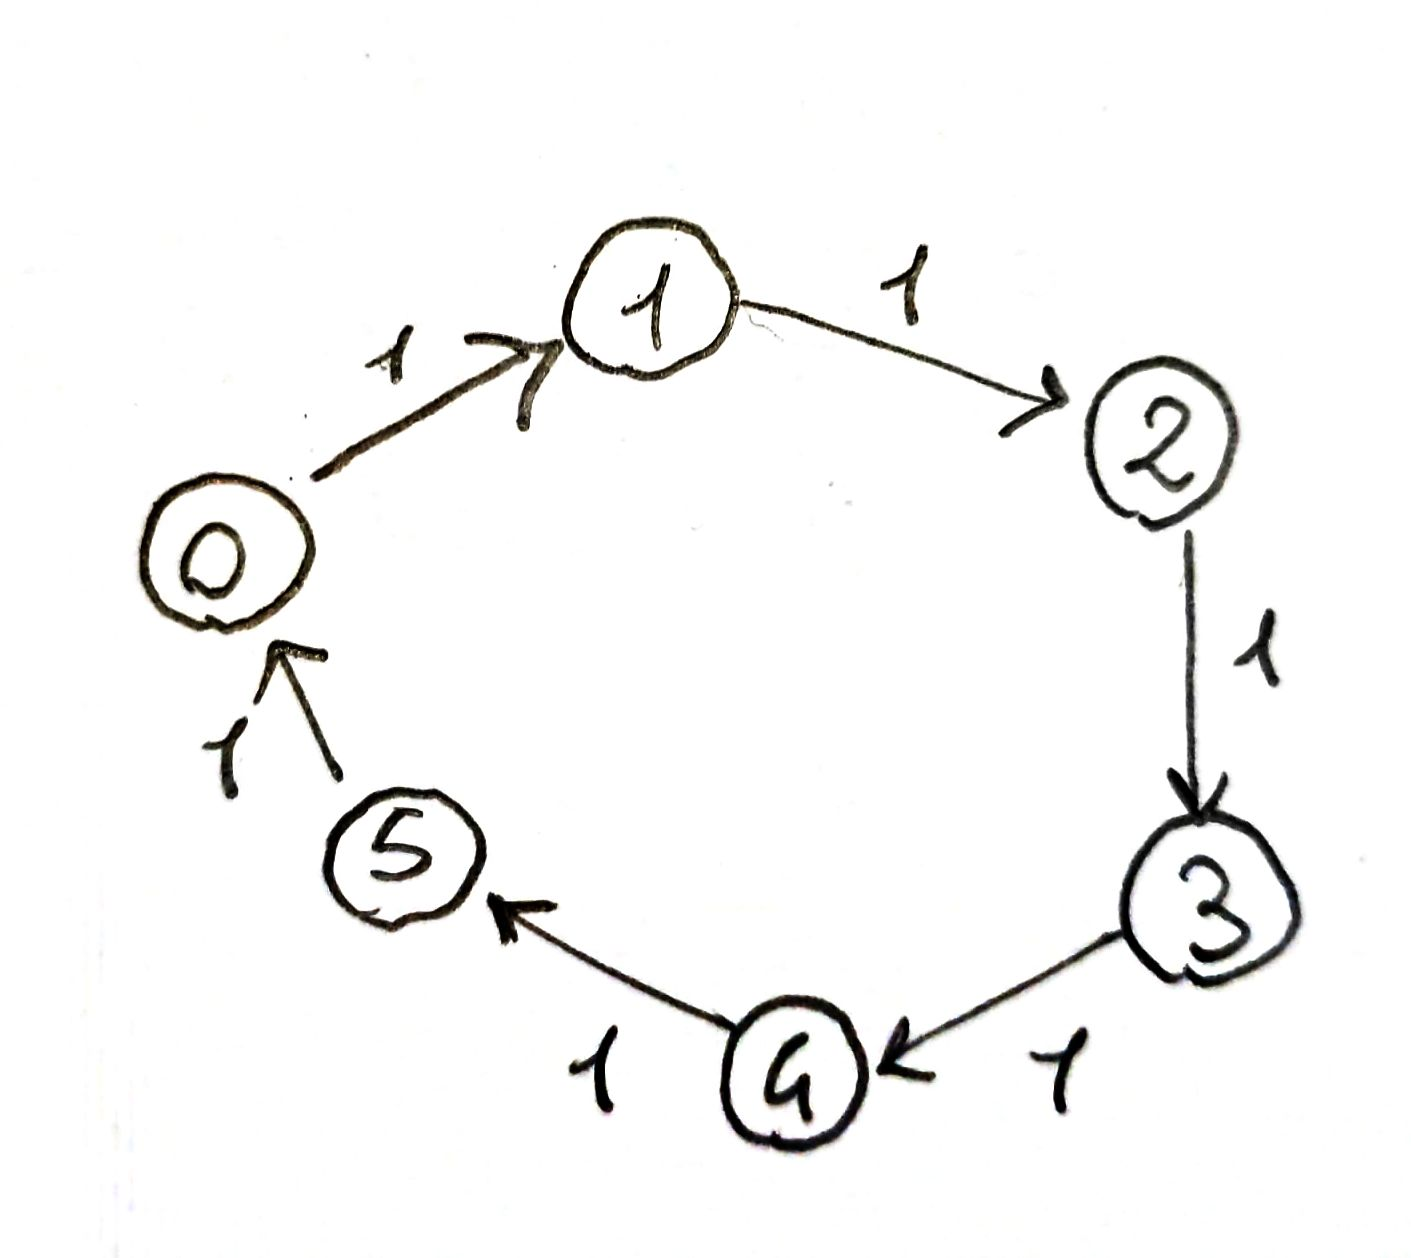
\includegraphics[width=0.4\textwidth]{Images/block-n.jpeg}
    \begin{tikzpicture}[shorten >=1pt,node distance=2cm,auto]
        \tikzstyle{every state}=[fill={rgb:black,1;white,10},font=\bfseries]
        \tikzset{every loop/.style={min distance=4mm,looseness=4}}
        \node[state] (q0) {0};
        \node[state, above right of=q0] (q1) {1};
        \node[state, below right of=q1] (q2) {2};
        \node[state, below right of=q2] (q3) {3};
        \node[state, below left of=q3] (q4) {4};
        \node[state, below right of=q0] (q5) {5};
        \path[->]
        (q0) edge [above left] node{$1$} (q1)
        (q1) edge [above] node{$1$} (q2)
        (q2) edge [above right] node{$1$} (q3)
        (q3) edge [below right] node{$1$} (q4)
        (q4) edge [below] node{$1$} (q5)
        (q5) edge [below left] node{$1$} (q0);
    \end{tikzpicture}
    \caption{Block diagram for a $N=6$ cyclic Markov chain}
    \label{fig:block-N}
\end{figure}
\end{comment}

The simplest way would be:
\begin{align*}
    \mathbb{P}(\mu \to \nu) = k \exp\left(-\frac{1}{Z} \beta(\mathcal{E}_\mu - \mathcal{E}_\nu) \right)
\end{align*}
but this is not computationally efficient, because most of the transitions occur with very low probabilities. 

\medskip

So we need a way to choose $\nu$ in an efficient manner. This is done with the \textbf{Metropolis algorithm}. The idea is to pick $\mu$ which is very similar to $\mu$. In the case of an Ising model, for example, this would amount to \textit{selecting} a spin in the initial state $\bm{s}$, and flipping it. The new state $\bm{s}'$ so obtained would be such that $\mathbb{P}(\mu \to \nu)$ is significant.

\medskip

Then $\mathbb{P}(\mu \to \nu) = g(\mu \to \nu) \mathcal{A}(\mu \to \nu)$, where $g(\mu \to \nu)$ is the probability of selecting $\nu$ starting from $\mu$ (for example the probability of flipping a certain spin in a set of $N$, which is $1/N$), and $\mathcal{A}(\mu \to \nu)$ is the \textit{acceptance} probability, i.e. the probability that the transition happens in the system. In the simple Ising model, the selection rule is time symmetric: $g(\mu \to \nu) = g(\nu \to \mu) = 1/N$. Then
\begin{align*}
    \frac{\mathbb{P}(\mu \to \nu)}{\mathbb{P}(\nu \to \mu)} = \frac{\frac{1}{N} \mathcal{A}(\mu \to \nu)}{\frac{1}{N} \mathcal{A}(\nu \to \mu)}  
\end{align*}
Following \textbf{Metropolis choice}:
\begin{align*}
    A(\mu \to \nu) = \begin{cases}
        e^{-\beta (\mathcal{E}_\nu - \mathcal{E}_\mu)} & \mathcal{E}_\nu > \mathcal{E}_\mu\\
        1 & \text{if } \mathcal{E}_\nu < \mathcal{E}_\mu
    \end{cases}
\end{align*}  
Note that:
\begin{align*}
    \frac{\mathcal{A}(\mu \to \nu)}{\mathcal{A}(\nu \to \mu)} = \begin{cases}
        e^{-\beta (\mathcal{E}_\nu - \mathcal{E}_\mu)} / 1 & \mathcal{E}_\nu > \mathcal{E}_\mu\\
        1/e^{-\beta (\mathcal{E}_\mu - \mathcal{E}_\nu)} & \mathcal{E}_\nu < \mathcal{E}_\mu
    \end{cases} = e^{-\beta (\mathcal{E}_\nu - \mathcal{E}_\mu)}
\end{align*}
and thus satisfies the detailed balance. 

\medskip

In more detail, for the Ising model with $h=0$ for simplicity, we have:
\begin{align*} %n.n. = nearest neighbour of i
    H = -\sum_{i,j = \mathrm{n.n.}(i) } J S_i S_j
\end{align*}
We start from a random configuration:
\begin{align*}
    \bm{s} = (s_1, s_2,\dots, s_N)
\end{align*}
And choose a new state $\bm{s}'$ by flipping a spin:
\begin{align*}
    \bm{s}' = (s_1, s_2, \dots, -s_k, \dots, s_N)
\end{align*}
Then:
\begin{align*}
    \mathcal{E}'-\mathcal{E}= [-J \sum_{J \in \mathrm{n.n}(k) } S_i S_J] ...
\end{align*}

...

Summarizing:
\begin{enumerate}
    \item Initialize the system
    \item Choose $k=1,\dots,N$ uniformly and compute $\Delta \mathcal{E}$
    \item If $\Delta \mathcal{E}< 0$, then accept the new state (flipping the $k$-th spin: $S_k \to -S_k$). If not, do the transition with probability $e^{-\beta \Delta \mathcal{E}}$. So:
    \begin{align*}
        \mathbb{P}(\mu \to \nu) = \min[1, e^{-\beta \Delta \mathcal{E}}]
    \end{align*}
    \item Repeat from $2$
\end{enumerate}

Note that this is a \textbf{local} algorithm, and so it is slow, especially for a large system, because changes take time to propagate. This is particularly significant near the critical temperature $T \approx T_c$, where the system becomes very slow (\textit{critical slowing down} phenomenon). So it would be more efficient to flip \textit{an entire cluster} of spins.

\medskip

This is the aim of \textbf{Wolff algorithm}. The idea is to \textit{build} a cluster of spins that are aligned:
\begin{itemize}
    \item Start from one spin at random
    \item Look at the neighbour with same spin, and add it to the cluster with probability $p$. Repeat over the neighbours until some spin is not accepted
    \item Flip the entire cluster
\end{itemize}

%See slides

  




%Complete drawing


\end{document}
